%----------
%	APLICABILIDAD EDITORIAL
%----------

Los resultados expuestos hasta aquí condicionan el modo en que este sistema puede
emplearse. El acuerdo con la anotación experta es limitado, y una parte de ese
desacuerdo obedece a la amplitud y variabilidad del criterio experto antes que a
un fallo de detección (Sección~\ref{sec:discussion}). El sistema no se plantea,
por tanto, como un clasificador autónomo, sino como un \textbf{apoyo a la
postedición} que se inserta en el flujo de trabajo de quien revisa un texto ya
redactado. Su cometido consiste en señalar las piezas candidatas y aportar en cada
caso las evidencias y la justificación del veredicto, de modo que la persona analista
acepte, rechace o matice ese diagnóstico con plena trazabilidad, en lugar de
partir de cero.

Para hacer efectiva esa aplicabilidad, el sistema de detección se ha integrado en
la \textbf{herramienta web del proyecto IRIS}~\cite{avi2026}\footnote{\url{https://dei.inf.uc3m.es/iris/} [Último acceso: 05/08/2026]},
lo que permite aplicarlo al conjunto del corpus, incluidas las miles de piezas que
carecen de anotación.

La asistencia cubre los dos planos del análisis de contenido experto
(Sección~\ref{sec:experts}). En el plano \textbf{cuantitativo}, la herramienta agrega
las etiquetas que produce el sistema en informes por variable, con tablas de
frecuencias y porcentajes sobre el conjunto seleccionado y un análisis descriptivo
automático (Figura~\ref{fig:iris-web-informe}), lo que permite explorar qué medios,
secciones o periodos concentran más usos marcados. En el plano \textbf{cualitativo},
para cada pieza muestra el marcado de las evidencias sobre el texto y la explicación
del veredicto (Figura~\ref{fig:iris-web-analisis}), de modo que quien analiza puede
examinar el fundamento de cada decisión.

Las Figuras~\ref{fig:iris-web-informe} y~\ref{fig:iris-web-analisis} ilustran ambas
vistas de la herramienta web, la de informe cuantitativo y la de análisis por pieza.
La validación de esta integración con redacciones reales, mediante estudios de uso
con profesionales, queda fuera del alcance de este trabajo y se plantea como línea
futura (Sección~\ref{sec:futurework_usecases}).

\begin{figure}[H]
    \centering
    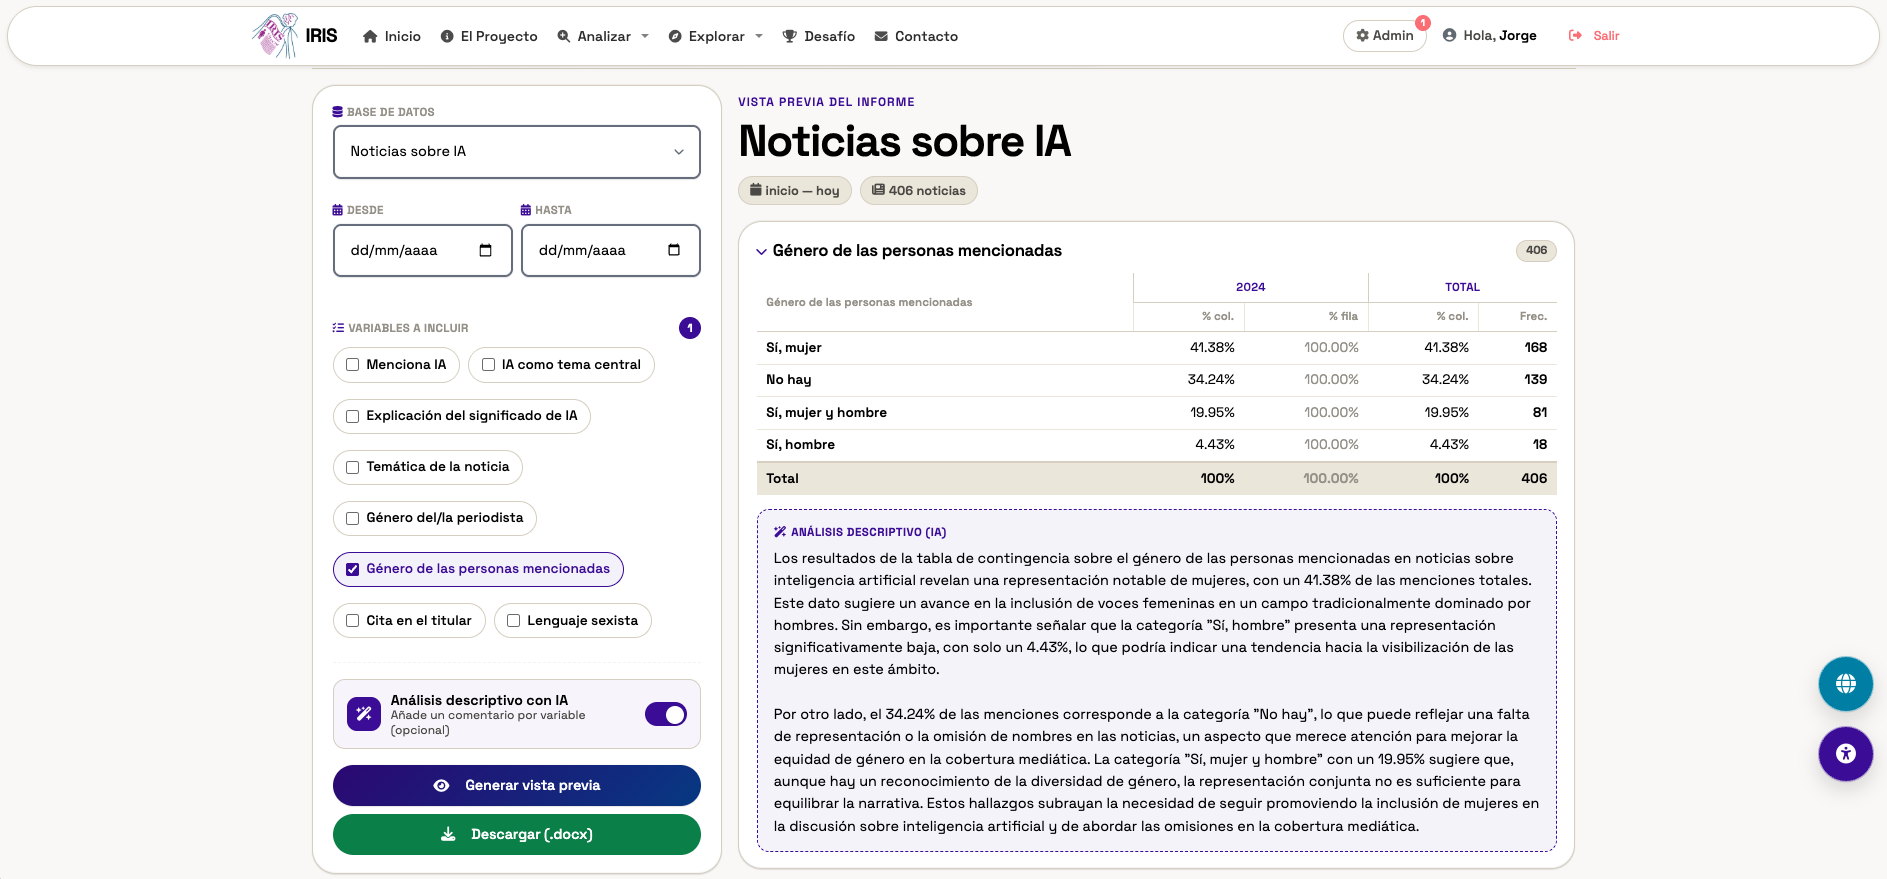
\includegraphics[width=\textwidth]{Plantilla_TFG_ingles_2019/imagenes/iris_3.png}
    \caption{Vista de informe cuantitativo en la herramienta web del proyecto IRIS.
    Para las variables seleccionadas genera tablas de frecuencias y porcentajes sobre
    el conjunto de piezas, acompañadas de un análisis descriptivo automático.}
    \label{fig:iris-web-informe}
\end{figure}

\begin{figure}[H]
    \centering
    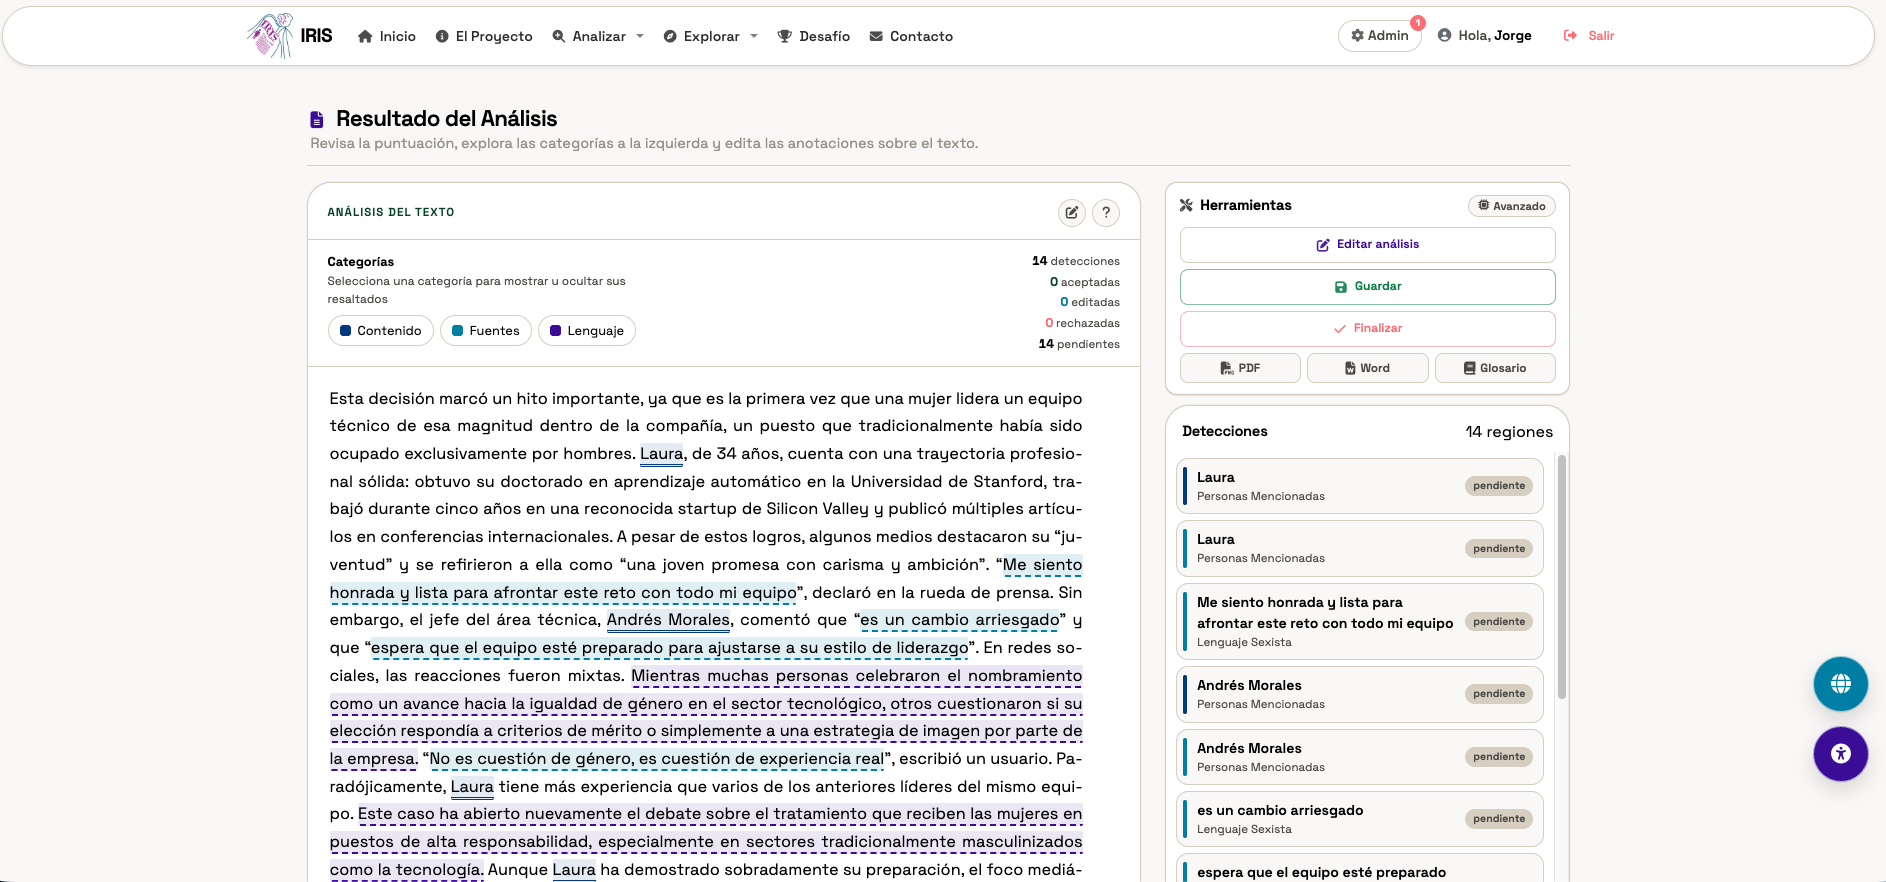
\includegraphics[width=\textwidth]{Plantilla_TFG_ingles_2019/imagenes/iris_2.png}
    \caption{Vista de resultado del análisis en la herramienta web del proyecto IRIS.
    Las detecciones se resaltan sobre el texto y se listan por categoría, con los
    controles para que la analista acepte, edite o rechace cada una (postedición con
    la persona en el bucle).}
    \label{fig:iris-web-analisis}
\end{figure}
